\documentclass[12pt,a4paper]{article}

\usepackage[utf8]{inputenc}
\usepackage[spanish]{babel}
\usepackage{palatino}
\usepackage{amsmath}
\usepackage{amssymb}
\usepackage{url}
\usepackage{hyperref}
\usepackage{enumerate}
\usepackage{geometry}
\usepackage{booktabs}
\usepackage{underscore}
\usepackage{longtable}
\usepackage{graphicx}
\usepackage{listings}

\geometry{
  a4paper,
  left=2.5cm,
  right=2.5cm,
  top=3cm,
  bottom=3cm
}

\begin{document}

\title{Análisis de Datos para Ciberseguridad: Trabajo práctico 1}

\author{
  Alonso Araya Calvo \\
  Pedro Soto \\
  Sofia Oviedo \\
  Instituto Tecnológico de Costa Rica, \\
  Escuela de Ingeniería en Computación, \\
  Programa de Maestría en Ciberseguridad
}

\date{ 24 de agosto de 2025 }
\maketitle

En este trabajo practico se realiza un análisis y implementación de un árbol de decisión para el set de datos KDD99.

Para efectos del proyecto se tomo un dataset reducido de KDD99, el cual contiene 10\% de los datos originales,
en el cual se va tomar en cuenta solamente las clases `normal' que indica tráfico normal y `backdoor' que indica tráfico malicioso.
Además de eso se creo una versión filtrada del dataset, sin duplicados, filas sin valores y datos categóricos convertidos a
numéricos mediante one-hot-encoding como lo son `protocol type', `service' y `flag'.

Se realizó un análisis de los momentos estadísticos de las características del dataset, así como el calculo de la distancia Jensen-Shannon,
histogramas comparativos y la creación, evaluación y análisis de un árbol de decisión.

Se utilizo librerías como numpy, pandas, matplotlib, scipy, pytorch y sklearn para los métodos creados para el trabajo.

\section{Análisis descriptivo de las características en el conjunto}\label{sec:analisis-descriptivo-de-las-caracteristicas-en-el-conjunto}

\subsection{Momentos estadísticos}\label{subsec:momentos-estadisticos}

Se calculó la media, desviación estándar, inclinación y kurtosis por medio de funciones de la librería pytorch.

Los resultados para el conjunto de datos de ataque y normal fueron los siguientes:

\begin{longtable}{lrrrr}
  \caption{Momentos Estadísticos para el set de ataque} \\
  \toprule
  & Media & Desviación Estándar & Inclinación & Kurtosis \\
  \midrule
  \endfirsthead
  \caption[]{Momentos Estadísticos para el set de ataque} \\
  \toprule
  & Media & Desviación Estándar & Inclinación & Kurtosis \\
  \midrule
  \endhead
  \midrule
  \multicolumn{5}{r}{Continua en la siguiente pagina} \\
  \midrule
  \endfoot
  \bottomrule
  \endlastfoot
  duration & 0.293388 & 1.660627 & 6.201858 & 39.309826 \\
  src_bytes & 53666.890625 & 4722.463867 & -6.375225 & 42.617065 \\
  dst_bytes & 8129.908203 & 919.138550 & -5.915853 & 35.871830 \\
  land & 0.000000 & 0.000000 & 0.000000 & -3.000000 \\
  wrong_fragment & 0.000000 & 0.000000 & 0.000000 & -3.000000 \\
  urgent & 0.000000 & 0.000000 & 0.000000 & -3.000000 \\
  hot & 1.917355 & 0.314076 & -3.661317 & 15.021400 \\
  num_failed_logins & 0.000000 & 0.000000 & 0.000000 & -3.000000 \\
  logged_in & 1.000000 & 0.000000 & 0.000000 & -3.000000 \\
  num_compromised & 0.924587 & 0.264193 & -3.210891 & 8.318419 \\
  root_shell & 0.000000 & 0.000000 & 0.000000 & -3.000000 \\
  su_attempted & 0.000000 & 0.000000 & 0.000000 & -3.000000 \\
  num_root & 0.000000 & 0.000000 & 0.000000 & -3.000000 \\
  num_file_creations & 0.000000 & 0.000000 & 0.000000 & -3.000000 \\
  num_shells & 0.000000 & 0.000000 & 0.000000 & -3.000000 \\
  num_access_files & 0.000000 & 0.000000 & 0.000000 & -3.000000 \\
  num_outbound_cmds & 0.000000 & 0.000000 & 0.000000 & -3.000000 \\
  is_host_login & 0.000000 & 0.000000 & 0.000000 & -3.000000 \\
  is_guest_login & 0.000000 & 0.000000 & 0.000000 & -3.000000 \\
  count & 3.524793 & 1.762356 & 2.291119 & 13.455750 \\
  srv_count & 3.829545 & 2.044711 & 2.924108 & 17.374548 \\
  serror_rate & 0.006002 & 0.047452 & 9.006940 & 85.688736 \\
  srv_serror_rate & 0.006519 & 0.048729 & 8.545023 & 77.689178 \\
  rerror_rate & 0.077944 & 0.174668 & 2.812351 & 9.046575 \\
  srv_rerror_rate & 0.133843 & 0.206010 & 1.671782 & 2.774177 \\
  same_srv_rate & 0.997717 & 0.024070 & -10.881998 & 121.573830 \\
  diff_srv_rate & 0.004587 & 0.048423 & 10.929219 & 122.999672 \\
  srv_diff_host_rate & 0.117965 & 0.243028 & 2.022636 & 3.229588 \\
  dst_host_count & 146.418396 & 90.726547 & -0.056618 & -1.562307 \\
  dst_host_srv_count & 146.418396 & 90.726547 & -0.056618 & -1.562307 \\
  dst_host_same_srv_rate & 1.000000 & 0.000000 & 0.000000 & -3.000000 \\
  dst_host_diff_srv_rate & 0.000000 & 0.000000 & 0.000000 & -3.000000 \\
  dst_host_same_src_port_rate & 0.023202 & 0.078893 & 9.197856 & 101.049896 \\
  dst_host_srv_diff_host_rate & 0.000000 & 0.000000 & 0.000000 & -3.000000 \\
  dst_host_serror_rate & 0.002035 & 0.005504 & 3.185214 & 11.143164 \\
  dst_host_srv_serror_rate & 0.002035 & 0.005504 & 3.185214 & 11.143164 \\
  dst_host_rerror_rate & 0.063564 & 0.110032 & 4.960103 & 31.944805 \\
  dst_host_srv_rerror_rate & 0.063564 & 0.110032 & 4.960103 & 31.944805 \\
  flag_OTH & 0.000000 & 0.000000 & 0.000000 & -3.000000 \\
  flag_REJ & 0.000000 & 0.000000 & 0.000000 & -3.000000 \\
  flag_RSTO & 0.000000 & 0.000000 & 0.000000 & -3.000000 \\
  flag_RSTR & 0.092975 & 0.290548 & 2.798880 & 5.839768 \\
  flag_S0 & 0.000000 & 0.000000 & 0.000000 & -3.000000 \\
  flag_S1 & 0.002066 & 0.045431 & 21.897779 & 478.006714 \\
  flag_S2 & 0.005165 & 0.071721 & 13.784595 & 188.209549 \\
  flag_S3 & 0.000000 & 0.000000 & 0.000000 & -3.000000 \\
  flag_SF & 0.899793 & 0.300431 & -2.658721 & 5.074041 \\
  protocol_type_icmp & 0.000000 & 0.000000 & 0.000000 & -3.000000 \\
  protocol_type_tcp & 1.000000 & 0.000000 & 0.000000 & -3.000000 \\
  protocol_type_udp & 0.000000 & 0.000000 & 0.000000 & -3.000000 \\
  service_IRC & 0.000000 & 0.000000 & 0.000000 & -3.000000 \\
  service_X11 & 0.000000 & 0.000000 & 0.000000 & -3.000000 \\
  service_auth & 0.000000 & 0.000000 & 0.000000 & -3.000000 \\
  service_domain & 0.000000 & 0.000000 & 0.000000 & -3.000000 \\
  service_domain_u & 0.000000 & 0.000000 & 0.000000 & -3.000000 \\
  service_eco_i & 0.000000 & 0.000000 & 0.000000 & -3.000000 \\
  service_ecr_i & 0.000000 & 0.000000 & 0.000000 & -3.000000 \\
  service_finger & 0.000000 & 0.000000 & 0.000000 & -3.000000 \\
  service_ftp & 0.000000 & 0.000000 & 0.000000 & -3.000000 \\
  service_ftp_data & 0.000000 & 0.000000 & 0.000000 & -3.000000 \\
  service_http & 1.000000 & 0.000000 & 0.000000 & -3.000000 \\
  service_ntp_u & 0.000000 & 0.000000 & 0.000000 & -3.000000 \\
  service_other & 0.000000 & 0.000000 & 0.000000 & -3.000000 \\
  service_pop_3 & 0.000000 & 0.000000 & 0.000000 & -3.000000 \\
  service_private & 0.000000 & 0.000000 & 0.000000 & -3.000000 \\
  service_red_i & 0.000000 & 0.000000 & 0.000000 & -3.000000 \\
  service_shell & 0.000000 & 0.000000 & 0.000000 & -3.000000 \\
  service_smtp & 0.000000 & 0.000000 & 0.000000 & -3.000000 \\
  service_ssh & 0.000000 & 0.000000 & 0.000000 & -3.000000 \\
  service_telnet & 0.000000 & 0.000000 & 0.000000 & -3.000000 \\
  service_tftp_u & 0.000000 & 0.000000 & 0.000000 & -3.000000 \\
  service_tim_i & 0.000000 & 0.000000 & 0.000000 & -3.000000 \\
  service_time & 0.000000 & 0.000000 & 0.000000 & -3.000000 \\
  service_urh_i & 0.000000 & 0.000000 & 0.000000 & -3.000000 \\
  service_urp_i & 0.000000 & 0.000000 & 0.000000 & -3.000000 \\
\end{longtable}

\begin{longtable}{lrrrr}
  \caption{Momentos Estadísticos para el set de tráfico normal} \\
  \toprule
  & Media & Desviación Estándar & Inclinación & Kurtosis \\
  \midrule
  \endfirsthead
  \caption[]{Momentos Estadísticos para el set de tráfico normal} \\
  \toprule
  & Media & Desviación Estándar & Inclinación & Kurtosis \\
  \midrule
  \endhead
  \midrule
  \multicolumn{5}{r}{Continua en la siguiente pagina} \\
  \midrule
  \endfoot
  \bottomrule
  \endlastfoot
  duration & 188.932388 & 1320.953003 & 10.840396 & 164.942474 \\
  src_bytes & 1270.249146 & 36017.765625 & 59.171658 & 3578.733887 \\
  dst_bytes & 3720.620850 & 39526.839844 & 70.640572 & 6578.882324 \\
  land & 0.000011 & 0.003374 & 296.354523 & 87825.000000 \\
  wrong_fragment & 0.000000 & 0.000000 & 0.000000 & -3.000000 \\
  urgent & 0.000034 & 0.010123 & 296.354523 & 87825.000000 \\
  hot & 0.049299 & 0.903317 & 24.367807 & 661.993713 \\
  num_failed_logins & 0.000205 & 0.021867 & 130.644180 & 19413.707031 \\
  logged_in & 0.792627 & 0.405427 & -1.443531 & 0.083783 \\
  num_compromised & 0.031606 & 4.258875 & 176.780899 & 33631.015625 \\
  root_shell & 0.000262 & 0.016180 & 61.770962 & 3813.695068 \\
  su_attempted & 0.000194 & 0.018170 & 100.561958 & 10543.062500 \\
  num_root & 0.062119 & 4.767146 & 176.494781 & 33756.796875 \\
  num_file_creations & 0.005226 & 0.213528 & 88.129669 & 9105.999023 \\
  num_shells & 0.000490 & 0.022121 & 45.161217 & 2037.558350 \\
  num_access_files & 0.005533 & 0.085450 & 26.301615 & 1401.320801 \\
  num_outbound_cmds & 0.000000 & 0.000000 & 0.000000 & -3.000000 \\
  is_host_login & 0.000000 & 0.000000 & 0.000000 & -3.000000 \\
  is_guest_login & 0.004224 & 0.064855 & 15.288565 & 231.742828 \\
  count & 8.850578 & 18.486605 & 9.788823 & 142.604019 \\
  srv_count & 11.906981 & 22.699772 & 7.060920 & 74.169861 \\
  serror_rate & 0.001757 & 0.029323 & 25.426783 & 760.219543 \\
  srv_serror_rate & 0.001987 & 0.027964 & 24.495110 & 742.421814 \\
  rerror_rate & 0.054141 & 0.225442 & 3.945983 & 13.596252 \\
  srv_rerror_rate & 0.054467 & 0.224103 & 3.948063 & 13.673273 \\
  same_srv_rate & 0.985932 & 0.090632 & -6.837379 & 47.955101 \\
  diff_srv_rate & 0.017889 & 0.115964 & 6.952574 & 49.550980 \\
  srv_diff_host_rate & 0.146088 & 0.287653 & 2.198094 & 3.573772 \\
  dst_host_count & 139.642456 & 102.324249 & -0.025722 & -1.709513 \\
  dst_host_srv_count & 203.544830 & 85.431877 & -1.390772 & 0.345991 \\
  dst_host_same_srv_rate & 0.853141 & 0.295919 & -1.947228 & 2.358836 \\
  dst_host_diff_srv_rate & 0.046478 & 0.155643 & 4.126388 & 16.291719 \\
  dst_host_same_src_port_rate & 0.122985 & 0.260985 & 2.556218 & 5.319210 \\
  dst_host_srv_diff_host_rate & 0.025484 & 0.049551 & 5.760909 & 61.377747 \\
  dst_host_serror_rate & 0.002349 & 0.030955 & 23.755972 & 625.237610 \\
  dst_host_srv_serror_rate & 0.001183 & 0.016544 & 43.771297 & 2172.942871 \\
  dst_host_rerror_rate & 0.056157 & 0.221028 & 3.890001 & 13.396219 \\
  dst_host_srv_rerror_rate & 0.054160 & 0.214456 & 3.889613 & 13.448563 \\
  flag_OTH & 0.000011 & 0.003374 & 296.354523 & 87825.000000 \\
  flag_REJ & 0.052999 & 0.224033 & 3.990454 & 13.923891 \\
  flag_RSTO & 0.000751 & 0.027402 & 36.438213 & 1325.758545 \\
  flag_RSTR & 0.000353 & 0.018784 & 53.199570 & 2828.226562 \\
  flag_S0 & 0.000581 & 0.024090 & 41.462498 & 1717.157349 \\
  flag_S1 & 0.000615 & 0.024788 & 40.292236 & 1621.482056 \\
  flag_S2 & 0.000194 & 0.013911 & 71.856895 & 5161.471680 \\
  flag_S3 & 0.000080 & 0.008927 & 112.000023 & 12542.145508 \\
  flag_SF & 0.944417 & 0.229117 & -3.879347 & 13.049479 \\
  protocol_type_icmp & 0.010156 & 0.100263 & 9.771049 & 93.474449 \\
  protocol_type_tcp & 0.862886 & 0.343970 & -2.109964 & 2.451977 \\
  protocol_type_udp & 0.126958 & 0.332928 & 2.240950 & 3.021888 \\
  service_IRC & 0.000478 & 0.021862 & 45.696457 & 2086.190186 \\
  service_X11 & 0.000102 & 0.010122 & 98.771362 & 9753.889648 \\
  service_auth & 0.002505 & 0.049985 & 19.905418 & 394.229889 \\
  service_domain & 0.000034 & 0.005844 & 171.094513 & 29271.669922 \\
  service_domain_u & 0.061754 & 0.240710 & 3.641234 & 11.258711 \\
  service_eco_i & 0.002915 & 0.053909 & 18.441393 & 338.088837 \\
  service_ecr_i & 0.002015 & 0.044846 & 22.208370 & 491.216827 \\
  service_finger & 0.005328 & 0.072801 & 13.589488 & 182.676331 \\
  service_ftp & 0.004247 & 0.065029 & 15.246999 & 230.473495 \\
  service_ftp_data & 0.043230 & 0.203376 & 4.491819 & 18.176649 \\
  service_http & 0.693176 & 0.461179 & -0.837738 & -1.298210 \\
  service_ntp_u & 0.003302 & 0.057366 & 17.316536 & 297.865479 \\
  service_other & 0.045940 & 0.209356 & 4.337631 & 16.815239 \\
  service_pop_3 & 0.000888 & 0.029787 & 33.511395 & 1121.026367 \\
  service_private & 0.016657 & 0.127983 & 7.553180 & 55.051144 \\
  service_red_i & 0.000011 & 0.003374 & 296.354523 & 87825.000000 \\
  service_shell & 0.000011 & 0.003374 & 296.354523 & 87825.000000 \\
  service_smtp & 0.109277 & 0.311988 & 2.504704 & 4.273590 \\
  service_ssh & 0.000011 & 0.003374 & 296.354523 & 87825.000000 \\
  service_telnet & 0.002493 & 0.049872 & 19.951149 & 396.052734 \\
  service_tftp_u & 0.000011 & 0.003374 & 296.354523 & 87825.000000 \\
  service_tim_i & 0.000023 & 0.004772 & 209.550690 & 43909.996094 \\
  service_time & 0.000398 & 0.019958 & 50.063965 & 2504.429199 \\
  service_urh_i & 0.000159 & 0.012624 & 79.186501 & 6268.572266 \\
  service_urp_i & 0.005032 & 0.070761 & 13.989758 & 193.715500 \\
\end{longtable}

Como se observan de las tablas anteriores es posible notar algunas diferencias entre las características.

En este caso se podrían destacar los siguientes puntos a continuación.

\subsubsection{Media}

\begin{itemize}
  \item La media de `duration' en el set de tráfico normal es mucho mayor que en el set de ataque.
    Indicando que las conexiones maliciosas son mucho más cortas.
  \item Los ataques de tipo `backdoor' envían una mayor cantidad de `src_bytes' y reciben una mayor cantidad de `dst_bytes' en promedio que las conexiones normales.
    Se podría decir que sugiere que los atacantes están enviando payloads maliciosos y extrayendo gran cantidad de datos.
  \item Se puede observar como `logged_in' tiene una media de uno en el set de ataque, lo que indica que las conexiones maliciosas se realizaron por medio de conexiones autenticadas.
  \item En el tráfico normal, características como `hot' y `num_compromised' tienen una media baja, lo que indica que en la mayoría de las conexiones normales no se intentan realizar acciones sospechosas al contrario de las conexiones maliciosas.
  \item Curiosamente en características como `su_attempted' y `num_root' tienen una media mayor en el tráfico normal que en el tráfico malicioso.
    Lo que podría indicar que los atacantes no intentan escalar privilegios o que lo hacen por otros medios, siendo un posible punto a investigar ya que lo común sería observar intentos de escalamiento de privilegios en el tráfico malicioso.
\end{itemize}

\subsubsection{Desviación Estándar}

\begin{itemize}
  \item En una gran mayoría de características, la desviación estándar es baja en el lado del tráfico de ataques, indicando que son más precisos y consistentes, dando paso a un patrón predecible para utilizar en un clasificador.
    Los ataques normales si presentan una desviación que indica que sus valores están distribuidos de manera más dispersa.
  \item En el lado normal es posible ver como casi ninguna desviación es 0, mientras que en el ataque existen una gran cantidad de características con valor de 0 o casi cero.
  \item Se da una gran desviación en el tráfico normal en características como `duration', `src_bytes' y `dst_bytes', lo que indica que las conexiones normales tienen una mayor variabilidad en su duración y en la cantidad de datos enviados y recibidos, siendo más `humana'.
\end{itemize}

\subsubsection{Inclinación}

\begin{itemize}
  \item En el tráfico normal existe una inclinación mucho más positiva que el tráfico maliciosos, tendiendo a tener una cola hacia la derecha.
    Es posible ver eso en campos como `duration', `src_bytes' y `dst_bytes'.
  \item En el tráfico malicioso, la inclinación tiende a ir cerca de cero o negativo, siendo distribuciones más concentradas en comparación al tráfico normal.
\end{itemize}

\subsubsection{Kurtosis}

\begin{itemize}
  \item El tráfico normal presenta una kurtosis alta en campos como `duration', `src_bytes' y `dst_bytes', lo que podría concluir que tiene picos más agudos y valores dispersos.
  \item El tráfico malicioso es más uniforme ya que la kurtosis es mucho más moderada.
\end{itemize}

\subsubsection{Conclusiones}

\begin{itemize}
  \item Los ataques de tipo backdoor son más constantes y precisos, sugiriendo que el tráfico se enfoca en realizar acciones por medio de automatizaciones y ataques similares generando un patrón que podría ser de uso para detectar ataques.
  \item Los ataques se concentran en áreas especificas por ejemplo el uso del servicio HTTP y protocolo TCP casi que exclusivamente siendo algo sospechoso al ver el tráfico normal y ver que utilizan una gran cantidad de servicios y protocolos.
  \item El tráfico normal dada su distribución dispersa se podría concluir que es indicadora de ser más `natural' y no parece generado por un atacante.
  \item Existen campos como `duration', `src_bytes', `dst_bytes', `logged_in' y `num_compromised', ademas de los diferentes servicios y protocolos, que se presentan como los campos más característicos por utilizar para poder realizar clasificaciones.
  \item Dada la diferencia y patrones reconocibles entre los diferentes tráficos se podría decir que esto es un buen candidato para un algoritmo de clasificación, dados sus patrones marcados.
\end{itemize}

\section{Histogramas y Distancia Jensen-Shannon}\label{sec:histogramas-y-distancia-jensen-shannon}

En esta parte del trabajo se realizo la generación de histogramas para todas las
características del dataset y se creo con los datos del dataset normal y
del dataset de ataque con el fin de poder observar diferencias entre los dos conjuntos de datos y sus campos.

Se utilizó un número de bins de 30 para todos los histogramas, con rangos normalizados
para asegurar comparabilidad entre las distribuciones de normal y backdoor.

Finalmente se calculo la distancia Jensen-Shannon entre los histogramas de los diferentes campos del dataset normal y del dataset de ataque,
y se genero una tabla con las distancias calculadas para cada campo.

\subsection{Histogramas}\label{subsec:histogramas}

Los histogramas fueron generados mediante la extracción de los valores de los dataframes de ataque y tráfico normal,
y se genero un histograma para cada campo mediante el uso de la función `hist' de matplotlib, además del uso
de la función `histogram' de numpy.

A continuación se muestran unos ejemplos de los histogramas generados para los campos `duration', `src_bytes' y `dst_bytes'.

\begin{figure}[htpb]
  \centering
  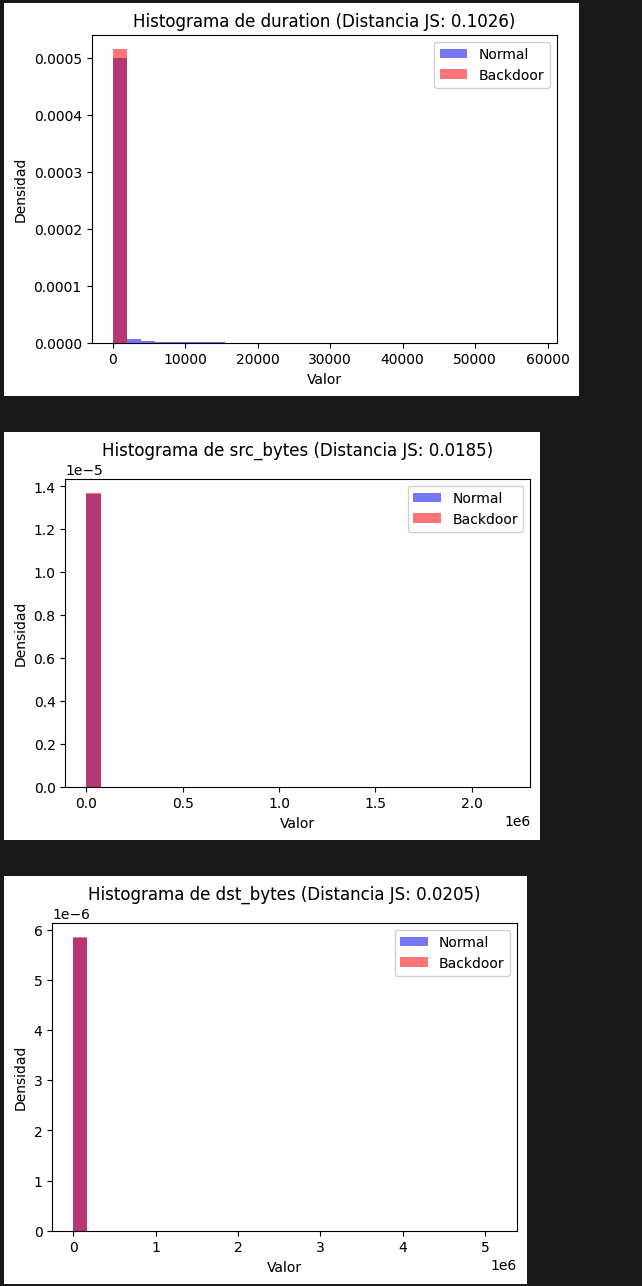
\includegraphics[width=0.4\textwidth]{images/histogramas}
  \caption{Histograma para el campo `duration', `src_bytes' y `dst_bytes'}\label{fig:figure}
\end{figure}

En el notebook de la solución se pueden apreciar todos los histogramas generados.

Como se observan en los histogramas presentados, existen características continuas como lo pueden ser
`duration', `src_bytes' y `dst_bytes' que presentan distribuciones con colas largas.
También existen características binarias como lo pueden ser `logged_in' que presentan distribuciones binarias en las que es posible ver
la diferencia entre el tráfico normal y el tráfico de ataques, así como los campos generados de los servicios y protocolos que muestran distribuciones discretas.
Además se puede observar como una gran cantidad de características presentan distribuciones asimétricas como
en el caso de campos que son de tipo conteos o tasas.

\subsection{Distancia Jensen-Shannon}\label{subsec:distancia-jensen-shannon}

\begin{longtable}{llr}
  \caption{Resumen de Distancias Jensen Shannon} \\
  \toprule
  & Feature & DistanciaJS \\
  \midrule
  \endfirsthead
  \caption[]{Resumen de Distancias Jensen Shannon} \\
  \toprule
  & Feature & DistanciaJS \\
  \midrule
  \endhead
  \midrule
  \multicolumn{3}{r}{Continua en la pagina siguiente} \\
  \midrule
  \endfoot
  \bottomrule
  \endlastfoot
  6 & hot & 0.813179 \\
  37 & dst_host_srv_rerror_rate & 0.466678 \\
  36 & dst_host_rerror_rate & 0.459732 \\
  24 & srv_rerror_rate & 0.373477 \\
  60 & service_http & 0.346864 \\
  30 & dst_host_same_srv_rate & 0.328221 \\
  29 & dst_host_srv_count & 0.298668 \\
  33 & dst_host_srv_diff_host_rate & 0.297726 \\
  27 & srv_diff_host_rate & 0.285225 \\
  23 & rerror_rate & 0.284472 \\
  8 & logged_in & 0.279071 \\
\end{longtable}

En la tabla anterior podemos ver una tabla resumida con los campos que contienen las mayores distancias Jensen-Shannon.
En el código de la implementación es posible ver la tabla completa pero se muestran los más significativos de ejemplo en este documento.
En este caso se muestran las 11 características con mayor distancia Jensen-Shannon.

Este numero nos ayuda a ver que tan diferentes son las distribuciones de los campos entre la clase normal y backdoor.

Como se aprecia en la tabla, el campo `hot' al tener una distancia alta, indica que las distribuciones son
muy diferentes entre la clase normal y la clase backdoor.

Las siguientes serian algunos campos de tipo de tasa de errores, se podría interpretar de esto que los ataques backdoor
generan tipos de errores que no son comunes en el tráfico normal, dada las acciones que realizan los ataques.

En cuanto a campos de servicios y protocolos, se muestran algunas con distancias moderadas y altas, como por ejemplo
`service_http' y protocolos como `tcp' y `udp' que muestran una distancia moderada indicando diferencias en el uso de los mismos.

Las características con distancia JS cerca de cero (como land, wrong_fragment, urgent)
fueron efectivamente identificadas como no discriminativas y podrían ser excluidas
del modelo sin pérdida de información relevante.

\subsection{Conclusiones}\label{subsec:conclusiones}

\begin{itemize}
  \item Mediante los histogramas y la distancia Jensen-Shannon es posible identificar las características que deberían ser tomadas como prioridad para el árbol de decisión, ya que son las más discriminativas.
  \item Características con duración de cero pueden ser eliminadas ya que no son necesarias al ser idénticas en ambos conjuntos y no proveer de datos útiles para el entrenamiento.
  \item Utilizar las características con una distancia alta podrían ser útiles a usar como umbral ya que podrían separar mejor las clases.
  \item Se denota que los ataques backdoor tienen como características más distintivas el uso de servicios como HTTP y protocolos como TCP, así como el valor `hot' y indicadores de error.
\end{itemize}

\section{Árbol de Decisión}\label{sec:arbol-de-decision}

En esta sección del trabajo se realizó la creación de las funciones más importantes para el arbol de decisión, como el calculo de Gini,
selección de características y creación de los nodos y hojas, así como pruebas unitarias para esta función.

\subsection{Calculo de Gini}\label{subsec:calculo-de-gini}

Para el calculo de Gini se utilizó la siguiente función:

    \begin{lstlisting}[language=Python, numbers=left,label={lst:lstlisting}, basicstyle=\ttfamily\tiny]
      def calculate_gini(self, data_partition_torch, num_classes=2):
        if data_partition_torch.numel() == 0:
            return 0.0

        class_counts = torch.bincount(data_partition_torch, minlength=num_classes).float()
        proportions = class_counts / class_counts.sum()
        gini_score = 1.0 - torch.sum(proportions ** 2)
        return gini_score.item()
    \end{lstlisting}

Esta función se encarga de calcular el coeficiente de Gini para una partición dada de un dataset y provista de un
numero de clases, en nuestro caso se deja de defecto el numero dos dado que se trabaja con normal y backdoor.

Se utiliza funciones de pytorch como `bincount' para contar las ocurrencias de cada clase en la partición y `sum' para obtener la suma de las ocurrencias
y sus proporciones al cuadrado, esto permite evitar el uso de bucles y se realiza una normalización matricial para obtener el resultado.
Además de esto se implementan protecciones ante valores anómalos como un tensor vació para evitar divisiones por cero.

Se realizan dos pruebas unitarias de esta manera:

    \begin{lstlisting}[language=Python, numbers=left,label={lst:lstlisting2}, basicstyle=\ttfamily\small]
      node = NodeCart(num_classes=2)
      ones_tensor = torch.tensor([1, 1, 1, 1])
      gini = node.calculate_gini(ones_tensor, num_classes=2)
      assert gini == 0.0, f"Se esperaba 0.0, se obtuvo {gini}"
      print("Test 1 Gini Pasado")

      variable_tensor = torch.tensor([0, 1, 2, 3])
      gini = node.calculate_gini(variable_tensor, num_classes=4)
      assert gini == 0.75, f"Se esperaba 0.75, se obtuvo {gini}"
      print("Test 2 Gini Pasado")
    \end{lstlisting}

La primera prueba se encarga de generar un tensor con valores de las mismas clases, esto con el fin de generar un Gini de 0
y poder verificar que el resultado es el esperado.

La segunda prueba es un tensor multiclase con lo que se espera un valor de 0.75 indicando la impureza para las cuatro clases.

Por medio de la función assert se verifica que el resultado es el esperado y se imprime un mensaje de éxito, si no este generaría
una exception de tipo AssertionError.

\subsection{Selección de Características}\label{subsec:seleccion-de-caracteristicas}

Para la selección de características se utilizo la siguiente función:

    \begin{lstlisting}[language=Python, numbers=left, basicstyle=\ttfamily\tiny,label={lst:lstlisting3}]
def select_best_feature_and_thresh(self, data_torch, num_classes=2):
      features = data_torch[:, :-1]
      labels = data_torch[:, -1].long()

      best_gini = float('inf')
      best_feature = None
      best_thresh = None

      for feature_idx in range(features.shape[1]):
          feature_values = features[:, feature_idx]
          unique_values = torch.unique(feature_values, sorted=True)

          for i in range(len(unique_values) - 1):
              threshold = (unique_values[i] + unique_values[i + 1]) / 2

              left_mask = feature_values < threshold
              right_mask = ~left_mask

              if left_mask.sum() == 0 or right_mask.sum() == 0:
                  continue

              left_labels = labels[left_mask]
              right_labels = labels[right_mask]

              weighted_gini = self.weighted_gini(left_labels, right_labels, num_classes)

              if weighted_gini < best_gini:
                  best_gini = weighted_gini
                  best_feature = feature_idx
                  best_thresh = threshold.item()

      return best_thresh, best_feature, best_gini
    \end{lstlisting}

La función se encarga de buscar todas las características disponibles y considerar todos los umbrales posibles.
Esta función utiliza solo bucles para iterar sobre las características y los umbrales posibles,
para realizar las iteraciones de manera eficiente se utiliza indexación lógica para crear las mascaras.
Además de eso también cuenta con medidas de protección ante división por cero o splits vacíos que no sirvan para el calculo.

Por medio del calculo de gini y sus promedios ponderados se busca el mejor umbral para la característica y se devuelve el mejor gini, característica y threshold encontrado.

\subsection{Ponderado de Gini}\label{subsec:ponderado-de-gini}

Para el ponderado de Gini se utilizo la siguiente función:

\begin{lstlisting}[language=Python, numbers=left, basicstyle=\ttfamily\tiny,label={lst:lstlisting4}]
def weighted_gini(self, left_side, right_side, num_classes=2):
    n = left_side.numel() + right_side.numel()
    if n == 0:
        return 0.0
    gini_left = self.calculate_gini(left_side, num_classes)
    gini_right = self.calculate_gini(right_side, num_classes)
    return (left_side.numel() / n) * gini_left + (right_side.numel() / n) * gini_right
\end{lstlisting}

Esta función calcula el gini ponderado por medio del uso de la función de calculo de gini mencionada anteriormente y el calculo mediante la formula
de ponderado proporcionada.
Se utiliza la función `numel' para obtener el numero de elementos de cada lado y se realiza la ponderación mediante la formula y los
datos obtenidos de la puntuación gini y el total de elementos.
Este recibe los datos de cada lado extraído dentro de la función de selección de características.

\subsection{Creación de Nodos y Hojas}\label{subsec:creacion-de-nodos-y-hojas}

Para la creación de nodos y hojas se utilizo la siguiente función:

    \begin{lstlisting}[language=Python, numbers=left, basicstyle=\ttfamily\tiny,label={lst:lstlisting5}]
  def create_with_children(self, data_torch, current_depth, min_gini=0.000001):
    labels = data_torch[:, -1].long()

    self.dominant_class = torch.mode(labels)[0].item()
    self.gini = self.calculate_gini(labels, self.num_classes)

    list_selected_features = []

    if (current_depth >= self.ref_cart.get_max_depth() or
            data_torch.shape[0] <= self.ref_cart.get_min_observations() or
            self.gini <= min_gini):
        return list_selected_features

    threshold, feature_idx, min_gini_split = self.select_best_feature_and_thresh(data_torch, self.num_classes)

    if feature_idx is None or min_gini_split >= self.gini:
        return list_selected_features

    self.feature_num = feature_idx
    self.threshold_value = threshold

    list_selected_features.append(feature_idx)

    features = data_torch[:, :-1]
    feature_values = features[:, feature_idx]

    left_mask = feature_values < threshold
    right_mask = ~left_mask

    left_data = data_torch[left_mask]
    right_data = data_torch[right_mask]

    if left_data.shape[0] > 0:
        self.node_left = NodeCart(self.num_classes, self.ref_cart, current_depth + 1)
        left_features = self.node_left.create_with_children(left_data, current_depth + 1, min_gini)
        list_selected_features.extend(left_features)

    if right_data.shape[0] > 0:
        self.node_right = NodeCart(self.num_classes, self.ref_cart, current_depth + 1)
        right_features = self.node_right.create_with_children(right_data, current_depth + 1, min_gini)
        list_selected_features.extend(right_features)

    return list_selected_features
    \end{lstlisting}

Esta función es la encargada de poder construir de manera recursiva el árbol de decisión, tiene dentro de ella
la lógica para determinar por medio de un conjunto de datos si debe crear alguna hoja o un nodo hijo.

Esta fase espera un tensor de pytorch la cual extrae la clase más frecuente para usarla
como clase dominante por medio de la función torch.mode
y se calcula el gini para el nodo.

Siguiendo con la función esta tiene como criterio de parada la profundidad máxima del arbol, si detecta un numero de muestras
menor al esperado o si el gini ya es lo suficientemente bajo, esto hace que se prevenga el overfitting y terminar
la función de una manera más inteligente.

Después de eso se busca la mejor partición mediante la búsqueda de la mejor característica y umbral, esta parte solo
va seguir dividiendo si se encuentra una mejor puntuación de gini, en caso contrario de no mejorar
se convierte en una hoja.

Además de eso se guarda valores como la característica y el umbral para poder usarlos en el árbol de decisión, y
guarda una lista de las características seleccionadas para poder usarlas en el árbol de decisión en sus proximas etapas.

En las partes finales se realiza la indexación lógica para generar la partición de los datos correctamente, se
crean hijos si contiene algún dato, genera nuevos objetos NodeCart para cada hijo y se llama nuevamente a la misma función
pero con un incremento de la profundidad, además de eso guarda todas las características utilizadas nuevamente
y las retorna cuando ya se cumple la función.

\subsection{Pruebas Unitarias}\label{subsec:pruebas-unitarias}

Para las pruebas unitarias se utilizaron las siguientes funciones:

\begin{itemize}
  \item test_select_best_feature_two_classes
  \item test_select_best_feature_single_class
  \item test_create_with_children_normal_splitting
  \item test_create_with_children_min_gini_condition
\end{itemize}

Para la función `test_select_best_feature_two_classes' lo que hace es buscar el mejor umbral
y característica para un tensor de dos clases. Se tiene una separación perfecta por lo que
se espera que se encuentre el umbral y característica correctos y que el gini sea 0 o mayor.
Así como validar que no se encuentren valores inválidos.

Para la función `test_select_best_feature_single_class' se busca el mejor umbral y característica para un tensor de una sola clase.
Ya que es una muestra que no tiene separación ya que solo hay una clase, se espera que no encuentre un posible umbral ni característica,
o si lo encuentra que Gini sea cero o similar pero sin ningún tipo de mejora al tener solo una clase.

Para la función `test_create_with_children_normal_splitting' se requiere construir correctamente un árbol con datos separables
y que este realmente encuentre una solución.
Para ello se provee de un tensor con clases distribuidas, para validar
el éxito se verifica si retorna una lista de características con al menos una, si el nodo raiz no es hoja,
si el nodo raíz tiene los valores de característica y umbral correctamente asignados y si existe algún hijo
de cualquier lado.

Para la función `test_create_with_children_min_gini_condition'
se busca crear un árbol de decisión
con un umbral minimo de gini, con el fin
de verificar si el parámetro funciona correctamente. Para ello se utiliza un tensor de la misma clase y una condición de parada
que debería activarse correctamente, en este caso no debería encontrar ningún nodo hijo y el nodo raíz debería ser una hoja,
por lo que se espera que no devuelva características y que el Gini sea menor al umbral que fue pasado por parámetros, así como
la clase dominante sea la esperada.

\subsection{Implementación de Test Cart}\label{subsec:implementacion-de-test-cart}

Para la implementación de test cart se utilizo la siguiente función:

    \begin{lstlisting}[language=Python, numbers=left, basicstyle=\ttfamily\small,label={lst:lstlisting9}]
  def test_cart(tree, testset_torch):
    if testset_torch.shape[0] == 0:
        return 0.0

    test_features = testset_torch[:, :-1]
    true_labels = testset_torch[:, -1].long()

    correct_predictions = 0
    total_predictions = testset_torch.shape[0]

    for i in range(total_predictions):
        current_observation = test_features[i]
        predicted_label = tree.evaluate_input(current_observation)
        true_label = true_labels[i].item()

        if predicted_label == true_label:
            correct_predictions += 1

    accuracy = correct_predictions / total_predictions
    return accuracy
    \end{lstlisting}

Esta función básicamente se encarga de evaluar el árbol de decisión con un conjunto de datos por medio del calculo de la métrica
de accuracy. Para ello la función extrae las características del tensor y sus clases, luego se realiza un bucle para evaluar cada observación
y se utiliza la función realizada en el código base `evaluate_input' para su evaluación, esta función se encarga de
analizar si es un nodo hoja y retornar la clase dominante o si es interno, evaluar a los diferentes hijos.
Para calcular el accuracy se utiliza la división entre el numero de predicciones correctas y el numero total de predicciones.

El accuracy lo que permite es medir el rendimiento del modelo y determinar si el árbol aprendió correctamente a poder clasificar
los casos que se le presenten, en caso contrario podría indicar overfitting, falta de entrenamiento o algún tipo de error que requiera
más entrenamiento, datos o ajustes al árbol.

Para las pruebas unitarias se realizaron dos las cuales fueron `test_cart_perfect_predictions' y `test_cart_invalid_dataset'.

La función `test_cart_perfect_predictions' se genera un set de datos de entrenamiento y prueba los cuales están formulados para que el resultado
sea una puntuación alta. El código nada más espera a que correctamente se devuelva algún accuracy entre cero y uno, esperando que
funcione correctamente.

La función `test_cart_invalid_dataset' lo que hace es por medio de un tensor con datos vacíos y uno con una sola observación,
verificar que el accuracy de un dataset vació es cero y que se maneje adecuadamente el caso de una sola observación por medio
de la verificación del accuracy retornado.

\section{Evaluación de CART}\label{sec:evaluacion-de-cart}

En este apartado se realiza el entrenamiento y pruebas de un árbol de decisión con el dataset KD999 bajo diferentes parámetros.

\subsection{Evaluación de máximo 3 y 4 nodos}\label{subsec:evaluacion-de-maximo-3-y-4-nodos}

El código utilizado para esta implementación se encuentra a continuación:

\begin{lstlisting}[language=Python, numbers=left, basicstyle=\ttfamily\tiny,label={lst:lstlisting9}]
  def get_cart_kd99_dataset_tensor():
    complete_dataset = pd.concat([df_no_attacks, df_attacks], ignore_index=True)

    class_mapping = {'normal.': 0, 'back.': 1}
    complete_dataset['outcome'] = complete_dataset['outcome'].map(class_mapping)

    dataset_tensor = torch.tensor(complete_dataset.values, dtype=torch.float32)

    print(f"\nDataset completo creado:")
    print(f"- Total de observaciones: {dataset_tensor.shape[0]}")
    print(f"- Numero de caracteristicas: {dataset_tensor.shape[1] - 1}")
    print(f"- Observaciones normales: {len(df_no_attacks)}")
    print(f"- Observaciones de backdoor: {len(df_attacks)}")
    print(f"- Distribucion de clases: {complete_dataset['outcome'].value_counts().to_dict()}")

    return dataset_tensor

def calculate_f1_score(y_true, y_pred, num_classes=2, print_results=False):
  f1_scores = []

  for class_id in range(num_classes):
      tp = torch.sum((y_true == class_id) & (y_pred == class_id)).float()
      fp = torch.sum((y_true != class_id) & (y_pred == class_id)).float()
      fn = torch.sum((y_true == class_id) & (y_pred != class_id)).float()

      precision = tp / (tp + fp) if (tp + fp) > 0 else torch.tensor(0.0)
      recall = tp / (tp + fn) if (tp + fn) > 0 else torch.tensor(0.0)

      f1 = 2 * (precision * recall) / (precision + recall) if (precision + recall) > 0 else torch.tensor(0.0)
      f1_scores.append(f1.item())

      if print_results:
          class_name = "Normal" if class_id == 0 else "Backdoor"
          print(f"- {class_name}: Precision={precision}, Recall={recall}, F1={f1}")

  return sum(f1_scores) / len(f1_scores)

  def evaluate_cart_complete(dataset_tensor, max_depth, min_observations=2):
    print(f"\n# Evaluacion de CART con profundidad maxima = {max_depth}")

    cart = CART(dataset_torch=dataset_tensor,
                max_cart_depth=max_depth,
                min_observations=min_observations)

    start_time = time.time()
    cart.build_cart(dataset_tensor)
    training_time = time.time() - start_time

    start_time = time.time()
    features = dataset_tensor[:, :-1]
    true_labels = dataset_tensor[:, -1].long()

    predicted_labels = []
    for i in range(features.shape[0]):
        prediction = cart.evaluate_input(features[i])
        predicted_labels.append(prediction)

    predicted_labels = torch.tensor(predicted_labels)
    evaluation_time = time.time() - start_time

    accuracy = test_cart(cart, dataset_tensor)

    print(f"Resultados por clase:")
    f1_score = calculate_f1_score(true_labels, predicted_labels, num_classes=2, print_results=True)

    print(f"\nResultados de corrida:")
    print(f"- Accuracy: {accuracy} ({accuracy * 100}%)")
    print(f"- F1-Score promedio: {f1_score}")
    print(f"- Tiempo de entrenamiento: {training_time} segundos")
    print(f"- Tiempo de evaluacion: {evaluation_time} segundos")
    print(f"- Caracteristicas seleccionadas: {len(cart.list_selected_features)}")
    print(f"- Features utilizadas: {cart.list_selected_features}")

    return {
        'accuracy': accuracy,
        'f1_score': f1_score,
        'training_time': training_time,
        'evaluation_time': evaluation_time,
        'selected_features': cart.list_selected_features,
        'cart': cart
    }

print(f"Datos de dataframes originales:")
print(f"- df_no_attacks (normal): {len(df_no_attacks)} observaciones")
print(f"- df_attacks (backdoor): {len(df_attacks)} observaciones")
print(f"- Clase en df_no_attacks: {df_no_attacks['outcome'].unique()}")
print(f"- Clase en df_attacks: {df_attacks['outcome'].unique()}")

complete_dataset = get_cart_kd99_dataset_tensor()

results_depth_3 = evaluate_cart_complete(complete_dataset, max_depth=3, min_observations=2)
results_depth_4 = evaluate_cart_complete(complete_dataset, max_depth=4, min_observations=2)

print(f"\nComparacion de resultados:")
print("=" * 60)
print(f"{'Metrica':<25} {'Profundidad 3':<15} {'Profundidad 4':<15}")
print("-" * 60)
print(f"{'Accuracy':<25} {results_depth_3['accuracy']:<15.4f} {results_depth_4['accuracy']:<15.4f}")
print(f"{'F1-Score':<25} {results_depth_3['f1_score']:<15.4f} {results_depth_4['f1_score']:<15.4f}")
print(
  f"{'Tiempo de Entrenamiento':<25} {results_depth_3['training_time']:<15.4f} {results_depth_4['training_time']:<15.4f}")
print(
  f"{'Tiempo de Evaluacion':<25} {results_depth_3['evaluation_time']:<15.4f} {results_depth_4['evaluation_time']:<15.4f}")
print(
  f"{'Features Seleccionadas':<25} {len(results_depth_3['selected_features']):<15}
   {len(results_depth_4['selected_features']):<15}")

print(f"\nResumen de mejores resultados:")
mejor_accuracy = "Profundidad 3" if results_depth_3['accuracy'] > results_depth_4['accuracy'] else "Profundidad 4"
mejor_f1 = "Profundidad 3" if results_depth_3['f1_score'] > results_depth_4['f1_score'] else "Profundidad 4"
print(f"- Mejor Accuracy: {mejor_accuracy}")
print(f"- Mejor F1-Score: {mejor_f1}")
\end{lstlisting}

Para esta prueba se desarrollo una implementación que genera nuevamente un dataset completo mediante la unión
de los dataframes de ataque y normal.
Lo siguiente seria realizar la evaluación de cada CART con los parámetros de profundidad máxima
3 y 4 y se reportan las métricas de accuracy, f1 score, tiempo de entrenamiento y evaluación, así como los features que
fueron utilizados para el entrenamiento.

Cabe recalcar que en esta función no se hizo ningún split de entrenamiento y prueba, por lo que si es posible realizar el proceso
de entrenamiento y evaluación, sin embargo al no realizar un split las pruebas no indican que tanto pueda generalizar a elementos
por los cuales no fue entrenado.

Para realizar esta parte primero se obtuvo el conjunto de datos completo en la función `get_cart_kd99_dataset_tensor'
que consiste de una union de los dataframes de ataque y normal, y
el mapeo de las clases en valores numéricos para poder convertirlo en un tensor de pytorch.

Para poder calcular el F1 Score se utilizo la función `calculate_f1_score' la cual se encarga de calcular
el F1 Score para cada clase.
Esta función evalúa cada clase por separado y genera las métricas de precision, recall y f1 score.
Siendo precisión la proporción de predicciones positivas, recall la proporción de casos positivos reales y el F1 siendo la media aritmética de precision y recall.
Para finalmente calcular la media simple de los F1 Score de ambas clases.

Para la función principal `evaluate_cart_complete' esta esta encargada de realizar la creación del árbol, entrenamiento, evaluación
bajo el mismo dataset, las predicciones para cada observación y el calculo de las métricas de evaluación. Esto es posible mediante
la construcción del objeto CART, los metodos `build_cart', `evaluate_input' y la función `test_cart' para obtener el accuracy, finalmente
se retorna las metricas obtenidas.

A continuación se muestra los resultados de una prueba realizada en Google Colab:

    \begin{lstlisting}[language=bash, numbers=left, basicstyle=\ttfamily\small,label={lst:lstlisting6}]
  Datos de dataframes originales:
  - df_no_attacks (normal): 87832 observaciones
  - df_attacks (backdoor): 968 observaciones
  - Clase en df_no_attacks: ['normal.']
  - Clase en df_attacks: ['back.']

  Dataset completo creado:
  - Total de observaciones: 88800
  - Numero de caracteristicas: 75
  - Observaciones normales: 87832
  - Observaciones de backdoor: 968
  - Distribucion de clases: {0: 87832, 1: 968}

  # Evaluacion de CART con profundidad maxima = 3
  Resultados por clase:
  - Normal: Precision=0.9999773502349854,
    Recall=0.9999886751174927, F1=0.999983012676239
  - Backdoor: Precision=0.997732400894165,
    Recall=0.9954751133918762, F1=0.996602475643158

  Resultados de corrida:
  - Accuracy: 0.9999662162162162 (99.99662162162161%)
  - F1-Score promedio: 0.9982927441596985
  - Tiempo de entrenamiento: 48.91265344619751 segundos
  - Tiempo de evaluacion: 1.4191524982452393 segundos
  - Caracteristicas seleccionadas: 4
  - Features utilizadas: [48, 1, 30, 1]

  # Evaluacion de CART con profundidad maxima = 4
  Resultados por clase:
  - Normal: Precision=0.9999773502349854,
    Recall=1.0, F1=0.9999886751174927
  - Backdoor: Precision=1.0,
    Recall=0.9954751133918762, F1=0.9977324604988098

  Resultados de corrida:
  - Accuracy: 0.9999774774774774 (99.99774774774775%)
  - F1-Score promedio: 0.9988605678081512
  - Tiempo de entrenamiento: 50.22194457054138 segundos
  - Tiempo de evaluacion: 1.3997457027435303 segundos
  - Caracteristicas seleccionadas: 6
  - Features utilizadas: [48, 1, 30, 1, 1, 36]

  Comparacion de resultados:
  ============================================================
  Metrica                   Profundidad 3   Profundidad 4
  ------------------------------------------------------------
  Accuracy                  1.0000          1.0000
  F1-Score                  0.9983          0.9989
  Tiempo de Entrenamiento   48.9127         50.2219
  Tiempo de Evaluacion      1.4192          1.3997
  Features Seleccionadas    4               6

  Resumen de mejores resultados:
  - Mejor Accuracy: Profundidad 4
  - Mejor F1-Score: Profundidad 4
    \end{lstlisting}

De los resultados anteriores se puede observar el nuevo dataset que contiene un total de 88800 observaciones, 75 características y
una distribución de clases de 87832 normales y 968 backdoor.

Finalmente se pudo determinar que en esta ejecución la profundidad cuatro contiene un mejor accuracy y F1 Score, con un tiempo de entrenamiento
de dos segundos mayor y un tiempo de evaluación similar, esto en contraste con la profundidad tres. Los resultados finalmente son muy similares,
inclusive el accuracy llega a ser 1 en ambos y el F1 diverge por un valor mínimo. Sin embargo si se utiliza más features en la profundidad cuatro que en la tres.
Además de eso el rendimiento es similar por lo que para este dataset es posible escoger elementos más profundos ya que no existe una diferencia de rendimiento
grande que pueda justificar el uso de una profundidad menor, aunque es posible si es necesario ya que el rendimiento es muy similar y para datasets mayores podría ser
beneficioso a nivel computacional usar una menor profundidad.

Esta función nos permite ver que el árbol y sus funciones de entrenamiento, evaluación y métricas funcionan correctamente, generando
datos útiles para poder mejorar el árbol y entender mejor que configuraciones y características son las mejores para este dataset, sin embargo se sabe que
es necesario poder realizar un split para poder asegurar su capacidad de generalización y concluir si existe overfitting o otros riesgos al árbol.

\subsection{Evaluación de profundidad 2 y 3, con particiones de entrenamiento y prueba}\label{subsec:evaluacion-de-profundidad-2-y-3-con-particiones-de-entrenamiento-y-prueba}

El código utilizado para esta implementación se encuentra a continuación:

\begin{lstlisting}[language=Python, numbers=left, basicstyle=\ttfamily\tiny,label={lst:lstlisting10}]
  def single_run_evaluation(dataset_tensor, max_depth, min_observations=2, random_state=None):
    if random_state is not None:
        torch.manual_seed(random_state)
        np.random.seed(random_state)
        random.seed(random_state)

    data_np = dataset_tensor.numpy()
    X = data_np[:, :-1]
    y = data_np[:, -1]

    X_train, X_test, y_train, y_test = train_test_split(
        X, y, test_size=0.3, random_state=random_state, stratify=y
    )

    train_tensor = torch.tensor(np.column_stack([X_train, y_train]), dtype=torch.float32)
    test_tensor = torch.tensor(np.column_stack([X_test, y_test]), dtype=torch.float32)

    cart = CART(dataset_torch=train_tensor,
                max_cart_depth=max_depth,
                min_observations=min_observations)

    start_time = time.time()
    cart.build_cart(train_tensor)
    training_time = time.time() - start_time

    start_time = time.time()
    accuracy = test_cart(cart, test_tensor)

    test_features = test_tensor[:, :-1]
    true_labels = test_tensor[:, -1].long()

    predicted_labels = []
    for i in range(test_features.shape[0]):
        prediction = cart.evaluate_input(test_features[i])
        predicted_labels.append(prediction)

    predicted_labels = torch.tensor(predicted_labels)
    evaluation_time = time.time() - start_time

    f1_score = calculate_f1_score(true_labels, predicted_labels, num_classes=2)

    return {
        'accuracy': accuracy,
        'f1_score': f1_score,
        'training_time': training_time,
        'evaluation_time': evaluation_time,
        'cart': cart,
        'train_size': train_tensor.shape[0],
        'test_size': test_tensor.shape[0]
    }

def evaluate_multiple_runs(dataset_tensor, max_depth, n_runs=10, min_observations=2):
  print(f"\nEjecutando {n_runs} corridas con profundidad maxima = {max_depth}:")
  results = []
  best_f1_idx = 0
  best_f1_score = -1

  for run in range(n_runs):
      print(f"- Corrida {run + 1}/{n_runs}...", end=" ")

      result = single_run_evaluation(
          dataset_tensor,
          max_depth,
          min_observations,
          random_state=42 + run
      )

      results.append(result)

      if result['f1_score'] > best_f1_score:
          best_f1_score = result['f1_score']
          best_f1_idx = run

      print(f"Acc: {result['accuracy']}, F1: {result['f1_score']}")

  accuracies = [r['accuracy'] for r in results]
  f1_scores = [r['f1_score'] for r in results]
  train_times = [r['training_time'] for r in results]
  eval_times = [r['evaluation_time'] for r in results]

  stats = {
      'accuracy_mean': np.mean(accuracies),
      'accuracy_std': np.std(accuracies),
      'f1_mean': np.mean(f1_scores),
      'f1_std': np.std(f1_scores),
      'train_time_mean': np.mean(train_times),
      'train_time_std': np.std(train_times),
      'eval_time_mean': np.mean(eval_times),
      'eval_time_std': np.std(eval_times),
      'best_run_idx': best_f1_idx,
      'best_cart': results[best_f1_idx]['cart'],
      'all_results': results
  }

  return stats

def display_results_table(stats_depth_2, stats_depth_3):
  print(f"\nTabla de resultados(Promedio y Desviacion Estandar)")
  print("=" * 80)
  print(f"{'Metrica':<25} {'Profundidad 2':<35} {'Profundidad 3'}")
  print("-" * 80)

  print(f"{'Accuracy':<25} "
        f"Promedio: {stats_depth_2['accuracy_mean']:.4f} y Desviacion: {stats_depth_2['accuracy_std']:.4f} "
        f"Promedio: {stats_depth_3['accuracy_mean']:.4f} y Desviacion: {stats_depth_3['accuracy_std']:.4f}")

  print(f"{'F1-Score':<25} "
        f"Promedio: {stats_depth_2['f1_mean']:.4f} y Desviacion: {stats_depth_2['f1_std']:.4f} "
        f"Promedio: {stats_depth_3['f1_mean']:.4f} y Desviacion: {stats_depth_3['f1_std']:.4f}")

  print(f"{'Tiempo de entrenamiento':<25} "
        f"Promedio: {stats_depth_2['train_time_mean']:.4f} y Desviacion: {stats_depth_2['train_time_std']:.4f} "
        f"Promedio: {stats_depth_3['train_time_mean']:.4f} y Desviacion: {stats_depth_3['train_time_std']:.4f}")

  print(f"{'Tiempo de evaluacion':<25} "
        f"Promedio: {stats_depth_2['eval_time_mean']:.4f} y Desviacion: {stats_depth_2['eval_time_std']:.4f} "
        f"Promedio: {stats_depth_3['eval_time_mean']:.4f} y Desviacion: {stats_depth_3['eval_time_std']:.4f}")

def generate_tree_visualization(cart, filename):
  xml_content = cart.to_xml(filename)
  print(f"- XML de arbol guardado en el archivo: {filename}")
  return xml_content

stats_depth_2 = evaluate_multiple_runs(complete_dataset, max_depth=2, n_runs=10, min_observations=2)
stats_depth_3 = evaluate_multiple_runs(complete_dataset, max_depth=3, n_runs=10, min_observations=2)

display_results_table(stats_depth_2, stats_depth_3)

print(f"\nMejores resultados:")
print(f"- Profundidad 2: Corrida {stats_depth_2['best_run_idx'] + 1} (F1-Score: {stats_depth_2['f1_mean']})")
print(f"- Profundidad 3: Corrida {stats_depth_3['best_run_idx'] + 1} (F1-Score: {stats_depth_3['f1_mean']})")

best_depth = 2 if stats_depth_2['f1_mean'] > stats_depth_3['f1_mean'] else 3

print(f"\nMejor profundidad general: {best_depth}")

print(f"\nGuardando arboles")

xml_file_depth_2 = f"mejor_arbol_profundidad_2.xml"
xml_file_depth_3 = f"mejor_arbol_profundidad_3.xml"

generate_tree_visualization(stats_depth_2['best_cart'], xml_file_depth_2)
generate_tree_visualization(stats_depth_3['best_cart'], xml_file_depth_3)
\end{lstlisting}

Para esta prueba se dividió el dataset en un 70\% de entrenamiento y 30\% de prueba, esto con el fin de poder
evaluar el árbol de decisión de una manera que se pueda comprobar su capacidad de generalización ante datos nunca antes vistos.

Además se realizan pruebas con 10 particiones aleatorias del conjunto de datos para una mayor verificación y una profundidad máxima de 2 y 3 nodos
con el fin de experimentar el rendimiento del árbol.
También se reportan las métricas necesarias como accuracy, F1 Score, tiempo de entrenamiento,
tiempo de evaluación, features seleccionadas y tiempo de ejecución, todo calculado por medio del promedio y la desviación estándar de todas las corridas.

Se generaron archivos XML que contienen la estructura de los arboles de decisión para cada mejor corrida, esto con el fin de poder visualizarlos.

En cuanto al código se desarrollaron multiples funciones para este efecto.
La función `single_run_evaluation' se encarga de realizar una corrida individual,
para ello se le pasa un tensor, la profundidad máxima, la cantidad de observaciones mínima y un estado aleatorio con el fin de
poder reproducir los experimentos si es lo deseado.
La función va a poder partir los datos por medio de la librería SciKitLearn y su función
train_test_split, esto con el fin de poder obtener los datos de entrenamiento y prueba, se convierten en tensores y se
llama a la función de `build_cart' y se construyen los objetos cart.
Después de ello se llama a `test_cart' para poder obtener el accuracy de la corrida y finalmente se generan
las predicciones para cada observación y se calcula el F1 Score, también la función retorna todas las métricas y el árbol para guardarlo
para su uso posterior.

En la función `evaluate_multiple_runs' se realiza el proceso de 10 corridas con diferentes particiones aleatorias del conjunto de datos,
esta función orquesta el uso de la función `single_run_evaluation' y se guardan los resultados en una lista, ademas de eso se calcula el mejor f1 score
gradualmente guardando el mejor F1 Score y el indice de la corrida que lo genero, reportando las métricas principales en stdout.
Esta función al terminar su corrida se genera una lista de los valores de accuracy, F1 y tiempos de evaluación y entrenamiento, generando los promedios y desviación de los
datos guardados en estas listas, los resultados de la mejor corrida y todos los resultados generales.

Finalmente el código en el notebook, se encarga de llamar a todas las funciones por medio de los parámetros requeridos como lo es
la profundidad esperada y el numero de corridas, se genera una tabla donde se observan mejor los resultados y se guardan en un XML
los mejores arboles para cada profundidad de la corrida.

En el siguiente bloque se muestran los resultados de una prueba realizada en Google Colab:

    \begin{lstlisting}[language=bash, numbers=left, basicstyle=\ttfamily\tiny,label={lst:lstlisting7}]
  Ejecutando 10 corridas con profundidad maxima = 2:
  - Corrida 1/10... Acc: 0.9998498498498498, F1: 0.992499589920044
  - Corrida 2/10... Acc: 0.9998873873873874, F1: 0.9943113327026367
  - Corrida 3/10... Acc: 0.9999624624624625, F1: 0.9981037676334381
  - Corrida 4/10... Acc: 0.9999624624624625, F1: 0.9981037676334381
  - Corrida 5/10... Acc: 0.9999624624624625, F1: 0.9981179237365723
  - Corrida 6/10... Acc: 0.9998873873873874, F1: 0.9943113327026367
  - Corrida 7/10... Acc: 0.9998873873873874, F1: 0.9943537712097168
  - Corrida 8/10... Acc: 0.9999624624624625, F1: 0.9981179237365723
  - Corrida 9/10... Acc: 1.0, F1: 1.0
  - Corrida 10/10... Acc: 0.9999624624624625, F1: 0.9981179237365723

  Ejecutando 10 corridas con profundidad maxima = 3:
  - Corrida 1/10... Acc: 0.9998498498498498, F1: 0.992499589920044
  - Corrida 2/10... Acc: 0.9998873873873874, F1: 0.9943113327026367
  - Corrida 3/10... Acc: 0.9999624624624625, F1: 0.9981037676334381
  - Corrida 4/10... Acc: 0.9999249249249249, F1: 0.9962217509746552
  - Corrida 5/10... Acc: 1.0, F1: 1.0
  - Corrida 6/10... Acc: 0.9999249249249249, F1: 0.9961932301521301
  - Corrida 7/10... Acc: 0.9998873873873874, F1: 0.9943537712097168
  - Corrida 8/10... Acc: 0.9999624624624625, F1: 0.9981179237365723
  - Corrida 9/10... Acc: 1.0, F1: 1.0
  - Corrida 10/10... Acc: 1.0, F1: 1.0

  Tabla de resultados(Promedio y Desviacion Estandar)
  ================================================================================
  Metrica                   Profundidad 2                         Profundidad 3
  --------------------------------------------------------------------------------
  Accuracy                  Promedio: 0.9999 y Desviacion: 0.0000 Promedio: 0.9999 y Desviacion: 0.0001
  F1-Score                  Promedio: 0.9966 y Desviacion: 0.0024 Promedio: 0.9970 y Desviacion: 0.0026
  Tiempo de entrenamiento   Promedio: 49.6658 y Desviacion: 0.1351 Promedio: 49.3974 y Desviacion: 0.6602
  Tiempo de evaluacion      Promedio: 1.0238 y Desviacion: 0.1602 Promedio: 1.0434 y Desviacion: 0.1286

  Mejores resultados:
  - Profundidad 2: Corrida 9 (F1-Score: 0.9966037333011627)
  - Profundidad 3: Corrida 5 (F1-Score: 0.9969801366329193)

  Mejor profundidad general: 3

  Guardando arboles
  - XML de arbol guardado en el archivo: mejor_arbol_profundidad_2.xml
  - XML de arbol guardado en el archivo: mejor_arbol_profundidad_3.xml
    \end{lstlisting}

De los resultados anteriores se observa que después de todas las corridas el mejor resultado es al utilizar la profundidad 3,
ya que este contiene el mejor accuracy y F1 Score promedio, sin embargo como se puede ver los resultados entre utilizar
profundidad 2 y 3 son muy similares, y no hay presencia de overfitting dando a entender que si es posible disceminar
entre tráfico normal y malicioso.
La unica salvedad es que la profunidad 3 utiliza más características que la 2.

Estos resultados con un dataset de entrenamiento aparte indican que el modelo si podría tener un buen resultado al tratar de generalizar,
ya que muchas corridas son casi perfectas y las validaciones generan muy poco margen de error.

Finalmente se genero un archivo XML de ambos nodos, a continuación se presenta un ejemplo del XML para el ejemplo de profundidad 3:

    \begin{lstlisting}[language=XML, numbers=left, basicstyle=\ttfamily\small,label={lst:lstlisting8}]
  <node>
    <thresh>0.5</thresh>
    <feature>48</feature>
    <depth>0</depth>
    <gini>0.009892582893371582</gini>
    <node>
      <thresh>64.5</thresh>
      <feature>1</feature>
      <depth>1</depth>
      <gini>0.49995195865631104</gini>
      <node>
        <thresh>373.5</thresh>
        <feature>1</feature>
        <depth>2</depth>
        <gini>0.012861132621765137</gini>
        <node>
          <thresh>0</thresh>
          <feature>0</feature>
          <depth>3</depth>
          <gini>0.0</gini>
          <dominant_class>0</dominant_class>
          <acc_dominant_class>None</acc_dominant_class>
    </node>
    <node>
      <thresh>0</thresh>
      <feature>0</feature>
      <depth>3</depth>
      <gini>0.006472349166870117</gini>
      <dominant_class>1</dominant_class>
      <acc_dominant_class>None</acc_dominant_class>
    </node>
    </node>
    <node>
      <thresh>0.004999999888241291</thresh>
      <feature>30</feature>
      <depth>2</depth>
      <gini>0.013114213943481445</gini>
      <node>
        <thresh>0</thresh>
        <feature>0</feature>
        <depth>3</depth>
        <gini>0.006622433662414551</gini>
        <dominant_class>0</dominant_class>
        <acc_dominant_class>None</acc_dominant_class>
      </node>
      <node>
        <thresh>0</thresh>
        <feature>0</feature>
        <depth>3</depth>
        <gini>0.5</gini>
        <dominant_class>0</dominant_class>
        <acc_dominant_class>None</acc_dominant_class>
      </node>
    </node>
  </node>
  <node>
    <thresh>0</thresh>
    <feature>0</feature>
    <depth>1</depth>
    <gini>0.0</gini>
    <dominant_class>0</dominant_class>
    <acc_dominant_class>None</acc_dominant_class>
  </node>
</node>
    \end{lstlisting}

El diagrama del árbol indica lo visto en los resultados, ya que es posible visualizar cuales features fueron
seleccionados para los diferentes nodos y su relevancia, también viendo los diferentes calculos, se puede observar
valores de Gini muy cercanos a cero, marcando que los splits son muy precisos.

En base a este árbol y la pregunta sobre el uso de Jensen-Shannon.
Se podría decir que al seguir los resultados previos de la tabla de distancias se podrían usar solo las
características que demuestren estar dentro de un rango específico y podrían reducir una gran cantidad de características,
esto dando el beneficio de manejar menos características y por ende un menor tiempo de entrenamiento y evaluación, así como
concentrarse en las características que realmente son relevantes para el modelo.

También otro beneficio es que al utilizar las características más significativas es posible que los splits sean más precisos
y se pueda tener una mejor solución al problema al encontrar los splits más rápido y con menos profundidad.

En el caso de realizar `early stopping' se puede utilizar esta distancia para determinar si es necesario seguir creando splits bajo características
que no proveen una ganancia significativa, esto con el fin de evitar overfitting por ejemplo.

Finalmente utilizar esta distancia de Jensen-Shannon podría proveer de arboles más eficientes, simples, efectivos y enfocado
en las características más relevantes para la tarea.
\end{document}